\documentclass{bioinfo}
\copyrightyear{2015} \pubyear{2015}

\access{Advance Access Publication Date: Day Month Year}
\appnotes{Manuscript Category}

\begin{document}
\firstpage{1}

\subtitle{Subject Section}

\title[short Title]{SSR-viz - a toolbox to detect and visualize protein
subfamily specific residues}
\author[Sample \textit{et~al}.]{Paul Zierep\,$^{\text{\sfb 1,}*}$, Stefan G\"unther\,$^{\text{\sfb 2}}$}
\address{$^{\text{\sf 1}}$Pharmaceutical Bioinformatics, Institute of Pharmaceutical Science, Albert-Ludwigs-University, Hermann-Herder-Strasse 9, Freiburg 79104, Germany. \\
%$^{\text{\sf 2}}$Department, Institution, City, Post Code, Country.
}

\corresp{$^\ast$To whom correspondence should be addressed.}

\history{Received on XXXXX; revised on XXXXX; accepted on XXXXX}

\editor{Associate Editor: XXXXXXX}

\abstract{
\textbf{Motivation:}
Protein subfamilies share a common structure but differ in functionalities such
as substrate specificity. These differences can often be assigned to a limited set 
of subfamily specific residues (SSRs). Often, only experimental evaluation, expert knowledge
and detailed protein structure investigation, reveal the correct assignment of these SSRs.
% Additionally, the detected SSRs which best distinguish two subfamily classes, 
% can be very different from the SSRs needed to distinguish another class.
% In cases such as nonribosomal peptide syntheses (NRPS), where dozens of subfamily classes can be defined,
% computational guidance becomes desirable. 
% Lastly, a general applicable algorithm to detect SSRs is difficult to define, as evolutionary distances 
% and general protein diversity require fine adjustment of any algorithm to distinguish true function 
% defining SSRs from merely random mutation. \\
Here, we introduce the toolbox SSR-viz, which allows 
to detect and visualize these SSRs
based on a multiple sequence alignment (MSA) and a file containing the subfamily class labels.  
The applied algorithm can be adjusted to
a given problem and allows users to perform a thorough analysis of their sequences. \\
% The toolbox can produce three different types of outputs which allow to further analyze the results: 
% First, an overview plot which is highly customizable and allows to visualize the SSRs of the entire 
% alignment, including general regions of interest. Secondly, a Jalview Annotation File, which allows
% to investigate the results together with the alignment in a sophisticated alignment editor. Finally,
% a summary CSV-file, which shows the conserved amino acid types in each class for highest scoring SSRs.
% This file allows the inclusion of protein structure indices, which makes it easy to investigate the found
% SSRs in an structural context. 
\textbf{Results:} Substrate specificity of non-ribosomal peptide synthases were analyzed.
The detected residues are located in the binding side and are in accordance with previous
performed studies.
\\
\textbf{Availability:} The toolbox is written as a GUI in Python3 and is available via
PyPi and the GitHub repository (https://github.com/PhaBiFreiburg/SSR-viz). Standalone executables are also available for 
Windows and Linux.
\\
\textbf{Contact:} \href{stefan.guenther@pharmazie.uni-freiburg.de }{stefan.guenther@pharmazie.uni-freiburg.de }\\
\textbf{Supplementary information:} Supplementary data are available at \textit{Bioinformatics}
online.} 

\maketitle

\section{Introduction}
\begin{figure*}[!tpb]%figure1
% \fboxsep=0pt\colorbox{gray}{
% \begin{minipage}[t]{235pt} \vbox to 100pt{\vfill\hbox to
% 235pt{\hfill\fontsize{24pt}{24pt}\selectfont FPO\hfill}\vfill}
% \end{minipage}}
%\centerline{
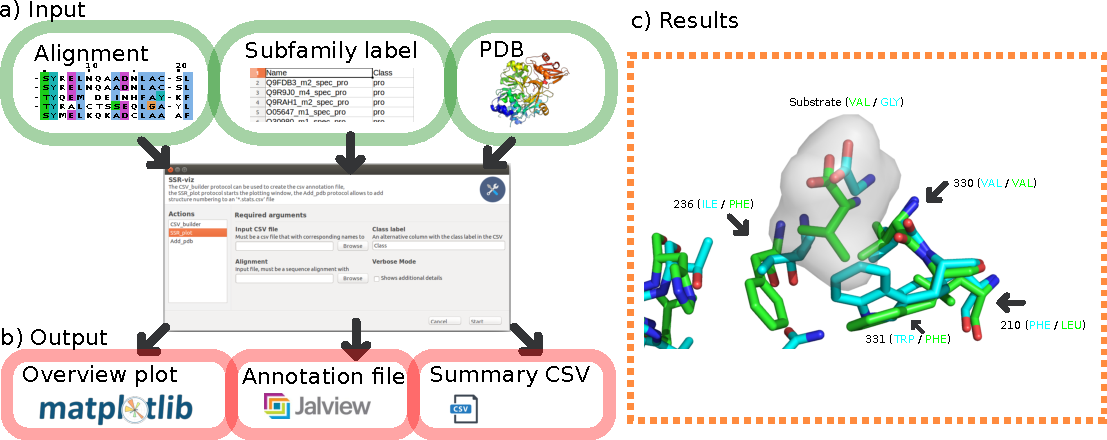
\includegraphics[width=\textwidth]{flow_chart} %}
\caption{General flow chart of the SSR-viz toolbox. a) The input consists 
of a MSA together with a CSV-file holding the corresponding subfamily class labels. 
Multiple protein structures can also be included in order to assign the 
structure indices. b) The output can be created as a mathplotlib PDF, a Jalview annotation file
or a summary CSV-File. This file is used to assign the indices of the structure.
c) Example assignment of SSRs for the NRPS adenylation domain with specificity for valine and glycine.   
}\label{fig:01}
\end{figure*}
Protein subfamilies differ from each other in very specific functions, such as substrate specificity,
protein-protein interaction or reaction type. These functionalities can often be assigned 
to a limited set of residues (referred to as subfamily specific residues (SSRs) in this article).
The identification of those SSRs is crucial to the understanding of protein subfamily diversity.
SSRs with high statistical significance can form the basis for various experiments 
such as side directed mutagenesis and rational design of proteins. \\
%to alter 
%proteins in their function or rational design experiments to design protein with totally new functionality.
%
Various approaches have been proposed to detect SSRs based on analysis of multiple sequence 
alignments (MSAs) of two or more protein subfamilies (\citealp{Hannenhalli01};\citealp{Edwards01};
\citealp{Olivera-Nappa01};\citealp{Suplatov01};\citealp{Suplatov02}). 
All these approaches share the 
common objective: to identify positions in the MSA which are conserved in one 
protein subfamily but differ between subfamilies. Some algorithms also include
physico-chemical properties of the residues in order to distinguish
true SSRs from residues which are due to evolutionary mutations. \\
%
In order to allow researchers a thorough study of their proteins we implemented an algorithm 
which follows this common objective but is also flexible and can be adjusted to a specific 
protein family observed. The algorithm allows the choice of various substitution matrices to define the similarity of residues.
The detection allows for three different kind of scoring modes: one-vs-one, which allows to detect SSRs most important to 
distinguish two subfamilies from each other; one-vs-all, which allows to detect SSRs most important to distinguish
one subfamily from a set of subfamilies and all-vs-all, which detects the most important residues to distinguish various 
subfamilies from each other.

Additionally, SSR-viz provides assistance for various tasks commonly encountered on the search for SSRs.
The main features are: The easy mapping of the alignment with a CSV-file which holds the information of 
the subfamily class labels. The addition of a window function, which allows to observe
single amino acid residues as well as general areas of interest in an alignment.
The residues can be mapped to a protein structure, which facilitates the
further investigation in a protein visualization tool such as PyMol (\citealp{schroedinger01}).
The creation of a Jalview (\citealp{clamp01}) annotation file which allows to integrate the results 
in the Jalview Alignment Editor together with the original alignment.
%
\section{Algorithm}
%
% \begin{equation}
% PPM =
% \left[ \begin{array}{cccc}
%   \alpha_{A1} & \alpha_{A2}  & ... & \alpha_{Am} \\
%   \alpha_{R1} & \alpha_{R2}  & ... & \alpha_{Rm} \\
%   ... & ... & ... & ...\\
%   \alpha_{n1} & \alpha_{n2}  & ... & \alpha_{nm} \\
% \end{array} \right]
% \end{equation}

% \begin{equation}
% EP(m) =
%   \begin{bmatrix}
%     \alpha_{A1} * \beta_{A1} & \alpha_{A1} * \beta_{R1} & ... & \alpha_{A1} * \beta_{n1} \\
%     \alpha_{R1} * \beta_{A1} & \alpha_{R1} * \beta_{R1} & ... & \alpha_{R1} * \beta_{n1} \\
%   ... & ... & ... & ...\\
%     \alpha_{n1} * \beta_{A1} & \alpha_{n1} * \beta_{R1} & ... & \alpha_{n1} * \beta_{n1} \\
%   \end{bmatrix}
% \end{equation}
%
Initially, each subfamily in the MSA is converted into a position 
probability matrix (PPM), which represents the probability to find a specific 
residue at a given position. This allows to compare the subfamilies 
independent of the number of their representing sequences. 
For each position (m) in the MSA the SSR score is computed based on the combination 
of three independent scoring functions (see Equation~(\ref{eq:01})).
%
\begin{equation}
\begin{aligned}
SSR_{score}(m) = & Conservation(m) * Difference(m) * \\ 
& Exchange(m) \label{eq:01} %\vspace*{-10pt}
\end{aligned}
\end{equation}  
%
The conservedness $Conservation(m)$ of each position is defined by the normalized Shannon entropy 
of both subfamilies. %(see Equation~(\ref{eq:01})).
%
% \begin{equation}
% S(m) = 1 - \frac{-\sum(\alpha_m*\log_2(\alpha_m))}{max(S(\alpha))} \label{eq:01} %\vspace*{-10pt}
% \end{equation}  
%
The difference $Difference(m)$ between two subfamilies is computed by summation of an exchange matrix. The matrix
represents the probability of each residue in one subfamily to be exchanged with another residue in 
the other subfamily. The more residues are exchanged the higher the score.
This matrix judges each amino acid exchange equally.
%
In order to differentiate the exchange of more divers amino acids,
an additional scoring function $Exchange(m)$ is implemented. 
Again, the exchange matrix is computed, but
this matrix can be weighed with a substitution matrix such as
PAM or BLOSSUM. A purely physico-chemical substitution matrix is also
available based on the research of \citealp{Chrysostomou01}.
%
A detailed explanation of the algorithm including an 
hypothetical example is given in the Supplementary data.
%\begin{methods}
\section{Implementation}
%
SSR-viz is based on a MSA as input, additionally a CSV-file is needed which supplies the 
subfamily specific label of each sequence. The CSV-File can be created using the
\textbf{CSV\_builder} tool. This tool allows also the label extraction from
the sequence name using regular expressions.
The CSV-file can have multiple labels, in case different types of functionality 
are investigated. The \textbf{CSV\_builder} also excludes redundant sequences by default.\\
%
The detection of SSRs is handled by the \textbf{SSR\_plot} tool. 
The detection threshold for SSRs can be assigned in two ways. Either the top N 
SSRs can be returned independent of their significance or the SSRs can be returned based
on their Z-score, which only returns positions that have a significant higher score then 
the other positions in the alignment. \\
%
SSR-viz supports three different kind of outputs:
A mathplotlib-style plot in PDF Format, which is customizable and consists
of a heatmap, which visualizes all the scores and a plot which shows the most 
significant SSRs. A window function can also be added to the plot, which allows 
to investigate the alignment for areas of general importance. \\
%
It is often desired to visualize the SSRs together with the MSA, therefore,
a Jalview annotation file can also be created, this file can be loaded into 
the Jalview Alignment Editor.\\
%
Finally, a summary CSV-file can be created, this file shows the SSRs
together with the conserved positions in each subfamily class. 
In order to investigate the SSRs in a structural context
another tool is implemented \textbf{Add\_pdb}, which allows for 
mapping of protein structure indices from a PDB file to the indices in the MSA.
\textbf{Add\_pdb} supports any PDB file, downloaded from PDB or custom exported from 
PyMol, as long as it can be aligned to the MSA.
A flow chart of the implementation is shown in Figure~1\vphantom{\ref{fig:01}}.

%\end{methods}

\section{Use case}

The toolbox was applied to detect SSRs for the adenylation domain of   
non-ribosomal peptide synthases (NRPS). 
The sequences and subfamily labels were extracted from the work of \citealp{Rausch01}.
The input and generated output files are available in the GitHub project,
including a detailed documentation which can help to reproduce the use 
case step-by-step. \\
Two subfamilies were chosen, with respective specificities 
for valine and glycine. 
For both subfamilies crystal structures are available (PDB: 3VNS, 4ZXI),
so that the detected SSRs can be interpreted in a structural context. 
The 10 most important SSRs to distinguish the two subfamilies from each other 
were calculated (using the default parameters of SSR-viz). 
Additionally, the most important SSRs
to distinguish all the subfamilies from each other (47 subfamiles, see supplementary data)
were also calculated. 
All SSRs were subsequently mapped to the structure investigated by \citealp{Stachelhaus01} (PDB: 1AMU), which allows for a
comparison with the described specificity-conferring code.
All described residues are numbered based on the 1AMU sequence. 
\\
%
% \begin{table}[!t]
% \processtable{10 most important SSRs to distinguish subfamilies with glycine and valine specificity and 
% all the subfamily classes \label{Tab:01}} 
% {\begin{tabular}{@{}lllllll@{}}\toprule G vs V & & & & All vs all &  \\
% Position  & Score & G cons. & V cons. & Position & Score \\\midrule
% 486 & 0.74& I & A & 486 & 0.59\\
% 749 & 0.70& W & F & 749 & 0.57\\
% 478 & 0.68& T & S & 739 & 0.56\\
% 601 & 0.66& W & F & 591 & 0.55\\
% 748 & 0.65& I & T & 490 & 0.54\\
% 591 & 0.64& Q & W & 478 & 0.53\\
% 592 & 0.62& A & L & 750 & 0.53\\
% 404 & 0.58& F & L & 601 & 0.52\\
% 403 & 0.58& N & R & 495 & 0.52\\
% 479 & 0.57& T & N & 476 & 0.51\\
% \botrule
% \end{tabular}}{Note: G cons. stands for the conserved residue for the subfamily with specificity for Glycine, The Positions are
% based on the alignment supplied in the supplementary data.}
% \end{table}
%
For the subfamilies with valine and glycine specificity all detected SSRs 
are in close proximity to the ligand (< 16 Angstrom, see supplementary Figure~1). The two most significant 
SSRs (236 and 331) flank the substrate binding side, which can explain the substrate choice due
to sterical interaction as shown in Figure~1\vphantom{\ref{fig:01}}. 

In the work of \citealp{Stachelhaus01}, the residues are divided into
highly variant and moderately variant residues. 
The highly variant residues show the highest flexibility 
with respect to substrate specificity.
All the highly variant residues are detected by the all-vs-all scoring mode
(239, 278, 299, 322, 331) in the top 10 SSRs.

For both scoring schemes only 5 SSRs overlap. Meaning, that they are equally important 
for distinguishing all the subfamilies from each other, as well as the two specifically 
observed families.
This highlights, that subfamilies can be defined in more detail,
by investigating SSRs independently for specific groups, then
trying to establish an overall code for all subfamilies.% specific code. 

% the 
% importance of a detailed subfamily specific investigation.

%
% Interestingly, the most significant position found by our analysis (486) is not 
% included in the Stachehauser code. Nevertheless, its key role can clearly be 
% derived from its position in the binding pocket (see supplementary data and Figure~1\vphantom{\ref{fig:01}}).
%
%
\section{Conclusion}
%
SSR-viz allows for a thorough analysis of protein subfamilies for SSRs based on different schemes and using 
various different substitution matrices. %Therefore, it can be adjusted to a specific protein family. 
The diversity of the output options allows to further analyze the SSRs together with the alignment or in a structural context. 
We hope, that SSR-viz will improve the understanding of protein subfamily diversity by allowing the 
thorough analysis of the responsible SSRs.
%
\section*{Funding}

This work has been supported by the German National Research Foundation [DFG, Research Training Group 1976].\vspace*{-12pt}

\bibliographystyle{natbib}
%\bibliographystyle{achemnat}
%\bibliographystyle{plainnat}
%\bibliographystyle{abbrv}
%\bibliographystyle{bioinformatics}
%
%\bibliographystyle{plain}
%
%\bibliography{Document}


\begin{thebibliography}{}
% 
\bibitem[Hannenhalli {\it et~al}., 2000]{Hannenhalli01}
Hannenhalli,S.S. and Russell,R.B. (2000) Analysis and prediction of functional sub-types from protein sequence alignments. {\it J. Mol. Biol.}, 303, 61-76.

\bibitem[Edwards {\it et~al}., 2005]{Edwards01}
Edwards,R.J. and Shields,D.C. (2005) BADASP: predicting functional specificity in protein families using ancestral sequences.{\it Bioinformatics}, 21, 4190-4191.

\bibitem[Olivera-Nappa {\it et~al}., 2011]{Olivera-Nappa01} 
Olivera-Nappa,A. et al. (2011) Mutagenesis Objective Search and Selection Tool (MOSST): an algorithm to predict structure-function related mutations in proteins. {\it BMC Bioinform.},  12, 122.

\bibitem[Suplatov {\it et~al}., 2014]{Suplatov01} 
Suplatov,D. et al. (2014) Zebra: a web server for bioinformatic analysis of diverse protein families. {\it J. Biomol. Struct. Dyn.}, 32, 1752-1758.

\bibitem[Suplatov {\it et~al}., 2015]{Suplatov02} 
Suplatov,D. et al. (2015) Robust enzyme design: bioinformatic tools for improved protein stability. {\it Biotechnol. J.}, 10, 344-355.

\bibitem[Schroedinger {\it et~al}., 2015]{schroedinger01}
Schrödinger, LLC (2015) The PyMOL Molecular Graphics System, Version 1.8.

\bibitem[Clamp {\it et~al}., 2004]{clamp01}
Clamp,M. et al. (2004) The Jalview Java alignment editor. {\it Bioinformatics}, 20, 426-427.

\bibitem[Chrysostomou {\it et~al}., 2015]{Chrysostomou01}
Chrysostomou,C. and Seker,H. (2015) Novel protein weight matrix generated from amino acid indices. In, 2015 37th Annual International Conference of the IEEE Engineering in Medicine and Biology Society (EMBC). 8181-8184.

\bibitem[Rausch {\it et~al}., 2005]{Rausch01}
Rausch,C. et al. (2005) Specificity prediction of adenylation domains in nonribosomal peptide synthetases (NRPS) using transductive support vector machines (TSVMs). {\it Nucleic Acids Res.}, 33, 5799-5808.

\bibitem[Stachelhaus {\it et~al}., 1999]{Stachelhaus01}
Stachelhaus,T. et al. (1999) The specificity-conferring code of adenylation domains in nonribosomal peptide synthetases. {\it Chem. Biol.}, 6, 493-505.
% \bibitem[Bofelli {\it et~al}., 2000]{Boffelli03}
% Bofelli,F., Name2, Name3 (2003) Article title, {\it Journal Name}, {\bf 199}, 133-154.
% 
% \bibitem[Bag {\it et~al}., 2001]{Bag01}
% Bag,M., Name2, Name3 (2001) Article title, {\it Journal Name}, {\bf 99}, 33-54.
% 
% \bibitem[Yoo \textit{et~al}., 2003]{Yoo03}
% Yoo,M.S. \textit{et~al}. (2003) Oxidative stress regulated genes
% in nigral dopaminergic neurnol cell: correlation with the known
% pathology in Parkinson's disease. \textit{Brain Res. Mol. Brain
% Res.}, \textbf{110}(Suppl. 1), 76--84.
% 
% \bibitem[Lehmann, 1986]{Leh86}
% Lehmann,E.L. (1986) Chapter title. \textit{Book Title}. Vol.~1, 2nd edn. Springer-Verlag, New York.
% 
% \bibitem[Crenshaw and Jones, 2003]{Cre03}
% Crenshaw, B.,III, and Jones, W.B.,Jr (2003) The future of clinical
% cancer management: one tumor, one chip. \textit{Bioinformatics},
% doi:10.1093/bioinformatics/btn000.
% 
% \bibitem[Auhtor \textit{et~al}. (2000)]{Aut00}
% Auhtor,A.B. \textit{et~al}. (2000) Chapter title. In Smith, A.C.
% (ed.), \textit{Book Title}, 2nd edn. Publisher, Location, Vol. 1, pp.
% ???--???.
% 
% \bibitem[Bardet, 1920]{Bar20}
% Bardet, G. (1920) Sur un syndrome d'obesite infantile avec
% polydactylie et retinite pigmentaire (contribution a l'etude des
% formes cliniques de l'obesite hypophysaire). PhD Thesis, name of
% institution, Paris, France.

\end{thebibliography}
\end{document}
